\documentclass{article}

% if you need to pass options to natbib, use, e.g.:
% \PassOptionsToPackage{numbers, compress}{natbib}
% before loading nips_2016
%
% to avoid loading the natbib package, add option nonatbib:
% \usepackage[nonatbib]{nips_2016}

\usepackage[final]{nips_2016}

% to compile a camera-ready version, add the [final] option, e.g.:
% \usepackage[final]{nips_2016}

\usepackage[utf8]{inputenc} % allow utf-8 input
\usepackage[T1]{fontenc}    % use 8-bit T1 fonts
\usepackage{hyperref}       % hyperlinks
\usepackage{url}            % simple URL typesetting
\usepackage{booktabs}       % professional-quality tables
\usepackage{amsfonts}       % blackboard math symbols
\usepackage{nicefrac}       % compact symbols for 1/2, etc.
\usepackage{microtype}      % microtypography
\usepackage{graphicx}
\usepackage{textcomp}
\newcommand{\quotes}[1]{``#1''}

\title{NBA game prediction based on historical data and injuries}

% The \author macro works with any number of authors. There are two
% commands used to separate the names and addresses of multiple
% authors: \And and \AND.
%
% Using \And between authors leaves it to LaTeX to determine where to
% break the lines. Using \AND forces a line break at that point. So,
% if LaTeX puts 3 of 4 authors names on the first line, and the last
% on the second line, try using \AND instead of \And before the third
% author name.
		
\author{
  Dionny Santiago\\
  Department of Computer Science\\
  Florida International University\\
  Miami, FL 33199 \\
  \texttt{dsant005@fiu.edu} \\
  %% examples of more authors
  \And
  Gregory Jean-Baptiste\\
  Department of Computer Science\\
  Florida International University\\
  Miami, FL 33199 \\
  \texttt{gjean011@fiu.edu} \\
  \And
  Xuejiao Liu\\
  Department of Computer Science\\
  Florida International University\\
  Miami, FL 33199 \\
  \texttt{xliu037@fiu.edu} \\
  %% \AND
  %% Coauthor \\
  %% Affiliation \\
  %% Address \\
  %% \texttt{email} \\
  %% \And
  %% Coauthor \\
  %% Affiliation \\
  %% Address \\
  %% \texttt{email} \\
  %% \And
  %% Coauthor \\
  %% Affiliation \\
  %% Address \\
  %% \texttt{email} \\
}

\begin{document}
% \nipsfinalcopy is no longer used

\maketitle

\begin{abstract}
  A popular use of machine learning principles is the prediction of outcomes in sporting events. Basketball, a popular sport in the United States, is the subject of many attempts to predict winners prior to matches. We attempt to match or surpass the accuracy of other attempts by identifying key features related to the outcomes of matches. Our experiments include a slew of machine learning algorithms, including ensemble methods. Additionally, we incorporate data related to player injuries as it relates to the performance of their teams in matches where they must be absent. We find that with available data, it is difficult exceed 70\% in accuracy for any algorithm. We also find that it is not enough to take note of missing players, and the importance of the missing players may be more related to the outcome of a match.
\end{abstract}

\section{Introduction}

Basketball is one the most popular games in the United States and also has much popularity abroad. It began as a simple gym exercise in the late 1800\textquotesingle s and slowly moved from high schools and into colleges. Finally, in the early 1950\textquotesingle s, the National Basketball Association (NBA) emerged as a major governing body of the professional version of the game. Ever since, the NBA has presided over a yearly tournament between official professional teams from all over North America. The annual tournament is called a season. During a season, each team competes against others several times and track their wins and losses. After a number of games (in the hundreds), the 16 teams with the most wins compete against each other in an elimination style tournament called the Playoffs. Playoff matches are best four out of seven. The team that wins the Playoffs wins the whole season. 

Our goal in this project is to attempt predicting the outcome of Basketball matches before they happen based on the characteristics of the two teams that are competing. While this may not be something that will benefit humanity in a great way, there a still some interesting applications of such predictions. For example, fantasy basketball is a virtual game where players can create teams based on real players and earn ranking based on the performance of their selected basketball players in real life. It may be beneficial for them to be able to predict how various teams will do and pick real players based on that. Fantasy Basketball, and fantasy sports in general generate millions a year. In fact, many researchers have studied this same topic [1][2][3][5][6].

\section{Related Work}

In "Prediction of NBA games based on Machine Learning Methods" [1], the goal is to survey several machine learning methods on a limited set of features. The major contributions were a great starting feature set starting point (although the data itself is not provided) for predicting NBA seasons 2006-2012. It was also determined that linear classifiers are particularly strong at NBA game prediction.

In "NBA Oracle" [2], once again several machine learning methods are used to predict NBA games of older seasons (1992-1996). While the first paper focused on team-centric features, this paper also dived into player-centric features. The paper also focuses on cluster analysis to predict optimal player positioning.

We explored several other approaches, for example: "A Multivariate Statistical Analysis of the NBA" [3] which also focused on exploring different basketball team/player features, and on statistical analysis rather than machine learning. Due to the limited amount of time for this project, we have decided to pursue different machine learning algorithms that have either not been mentioned in the research we looked at, or not applied to the specific seasons we are looking at. In addition, we are choosing to focus solely on team-centric data, once again due to time constraints.

\section{Technical Description}

Before a strategy for training and testing on classifiers could be devised, the relevant data had to be collected. The official API for raw NBA statistics is not free for developer, so an alternate data source was found at stats.nba.com/stats. The exposed API was undocumented except for a single post by an unknown developer, containing incomplete information about the end points and the available data. It took a considerable amount of time to go over the API and filter out data that was not useful. The resulting data consisted of individual game statistics, information about active teams based on the year and information about individual players. In its original format, there was not much that could be done with the data for machine learning purposes, so other metrics were devised based on what was available.

\subsection{Derived Metrics}

The first derived metric is the win/loss percentage for both teams, which is the total amount of victories over the total number of prior games played. This feature provides a general view of how a team performs. A team that wins more than it loses is typically expected to do well in any game with a reasonable probability of winning. The next metric is the average point differential. Even when a team wins or loses, it may be important to know how much the difference in scores was. For example, a team that consistently wins by a small margin needs to be fairly compared to a team that loses more often but wins by larger margins and loses by small margins. We take the average of the the difference for each team for all previous games. When a team wins, the difference is positive. In the event of a loss, the difference is negative. Next is the win percentage over the 8 games prior to the current one. Above, the overall win/loss percentage was discussed, but that does not account for fluctuations in performance over time. A team that usually does well may have a period of low performance for some reason. This can be captured by focusing on their most recent games, which could more reliably predict their performance in the current game. Next is the win/loss percentage as both a home team and a visiting team. In basketball, the home team is the team playing in the city they represent. The visiting team is the team playing outside of their city. Team performance can vary depending on whether or not they are playing home. One possible explanation is the level of moral support a team receives when playing at home versus playing away. While the reason is not clear, the effect is noticeable in many sports, so that feature is included. The inspiration for these features were drawn for other papers available online [1]. 

\subsection {Injury Data}

One last feature that was included was injury count. Every team usually has one or two \quotes{star} players who on average perform better than the rest of their teammates. The presence of these players drive the performance of the whole team, so the outcome of a single game can be determined by whether or not the star players are present. It would be beneficial to know if any members of the current team are injured and cannot participate in a match. http://www.prosportstransactions.com/basketball/ provides details about when players are injured and when they recover, at which point they would once again be able to play. The data is presented in tables through html, but no api is provided. It would have been too time consuming to manually copy the necessary data from the site into the necessary formats. A web crawler was developed that reads the data from the web pages, extracts relevant information and stores it in a database for later processing. The data consisted of the player name, team, date and the status of the injury (suspended for injury, or reinstated after recovery). Afterwards, a separate script was written that finds out which players played for which teams for each season. That is very important because players can be traded to different teams in between seasons. Players can also be drafted or retired. Once the team composition data was available, the date of a particular game could be used to find every player on the team. For each player, an injury date that is less than or equal to the date of the game was looked up. If it was a suspension, the player could not have been available to play. At the time, it was unclear whether this information would make a difference or not.

Using these features, a single data source was compiled that could be used for training and testing classifiers. In order to learn as much as possible about the interaction between the format of the data and the machine learning algorithms, several algorithms were trained and tested simultaneously. 

\subsection {Hyperparameter Tuning}

For the nearest neighbors algorithms, five different values were used for K based on hyperparameter tuning (3, 5, 7, 15, 40). K-Nearest Neighbors works by classifying examples based on their \quotes{distance} from similar training points. It is up to the user to decide how many training points to take into account when calculating distances. If K is too small, noise may have too much of an impact on testing. If K is too large, then the classification will be polluted by training points that are not similar to the example at all. We used Linear Regression and two Decision Tree algorithms, J48 and the Logistic Model Tree (LMT). The Logistic Model Tree combines decision tree principles and linear regression by employing linear regression models at its leaves. For ensemble, we used both AdaBoost, which adaptively trains its models based on incorrect predictions, and a standard ensemble method that uses majority voting. Additionally, we employed a Naive Bayes classifier. In order to tune the hyperparameters, cross-validation was employed. 

\subsection {Implementation Details}

In order to implement these experiments, we used a variety of tools. First and foremost, we used MongoDB, an open source NoSQL database software to store and manipulate our data. It is schemaless, which works well because we did not know how the data would be structured ahead of time. We used Node JS to implement the scripts that would collect the data and store it in the database. Node JS is a javascript framework for writing server side javascript programs and is supported by a slew of libraries that make many complicated tasks simple. That includes javascript implementations of machine learning algorithms. Most notably, our SVM experiments employed a Node JS library. The SVM was configured to perform many iterations in order to find the optimal hyperparameters for a given training and test set. However, not all of our needs could be satisfied from the Node JS libraries. The other tool that we were most familiar with was Weka, so we decided to use it to fill the gaps [4]. Manually using Weka to perform experiments would take too long and be error prone. Instead, a Weka adapter was developed that could interface with Weka through commands. Now we could treat Weka like another library in our scripts, leading to many opportunities for automating repetitive tasks and concurrently running experiments. 

A few papers of related work revealed that many testers used data points from training set in their test sets. This cannot accurate because the model would have future data that will make it appear more accurate than it actually is. Instead, three different methods of training were devised along the course of the project based on some observations. Initially, for testing on any season, the entire previous season was used for training. Later on, it was observed that changing the amount of historical data used for training affected the performance of the classifiers, where some became more accurate and others became less accurate; specifically, using the K most recent past matches for training as opposed to the entire last season. Every time a new test point was submitted, it would become a training point for the next test point. Then, the oldest game of the last season was disposed. The idea is that the most recent games could possibly be the best indicator of current team performance, while older data may be too old and not reflective of the current state of the team at all. Finally, a third training method was devised that included the injury data, which the first two strategies did not have. All three methods were examined using machine learning to determine which gave the best accuracy. 

\section{Experimental Results}

As mentioned earlier, we ran 3 major sets of experiments, and for each set, seasons 2011 - 2015 were examined. Here, we will present and discuss the results. 

First, we present the results of training classifiers on a portion of last seasons data to test the new season. For 2011, the best algorithm was the SVM with an accuracy of 65.8\%. In 2012 it was the Naive Bayes with an accuracy of 67.2\%. In 2013, the best algorithm again was the Naive Bayes with 65.4. In 2014, Linear Regression yielded the best accuracy with 68.3\%. Finally, in 2015 the SVM tied the LMT with an accuracy of 67.4\%. The first observation we make here is that the Naive Bayes algorithm performed consistently well over the course of the seasons. However, Linear Regression, SVM and LMT also performed well with regards to this set of experiments. In general, the predictions improved overall as the years advance because there is more historical data available for training.

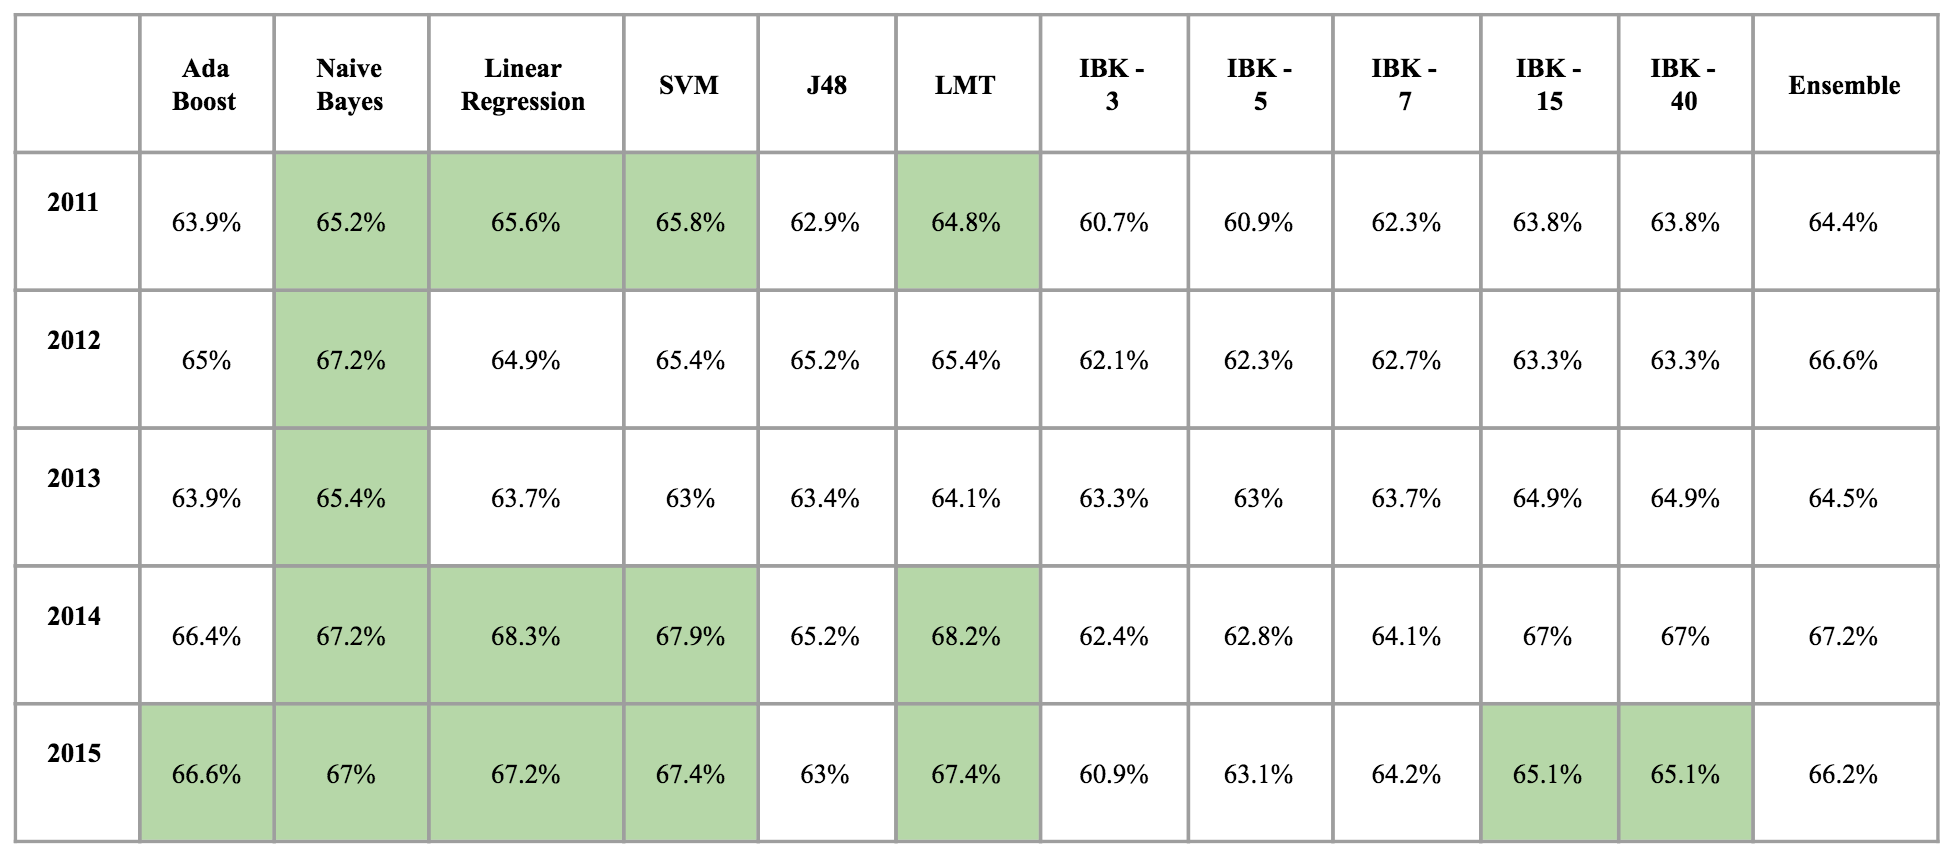
\includegraphics[scale=0.405]{images/partialPrevResults.png}

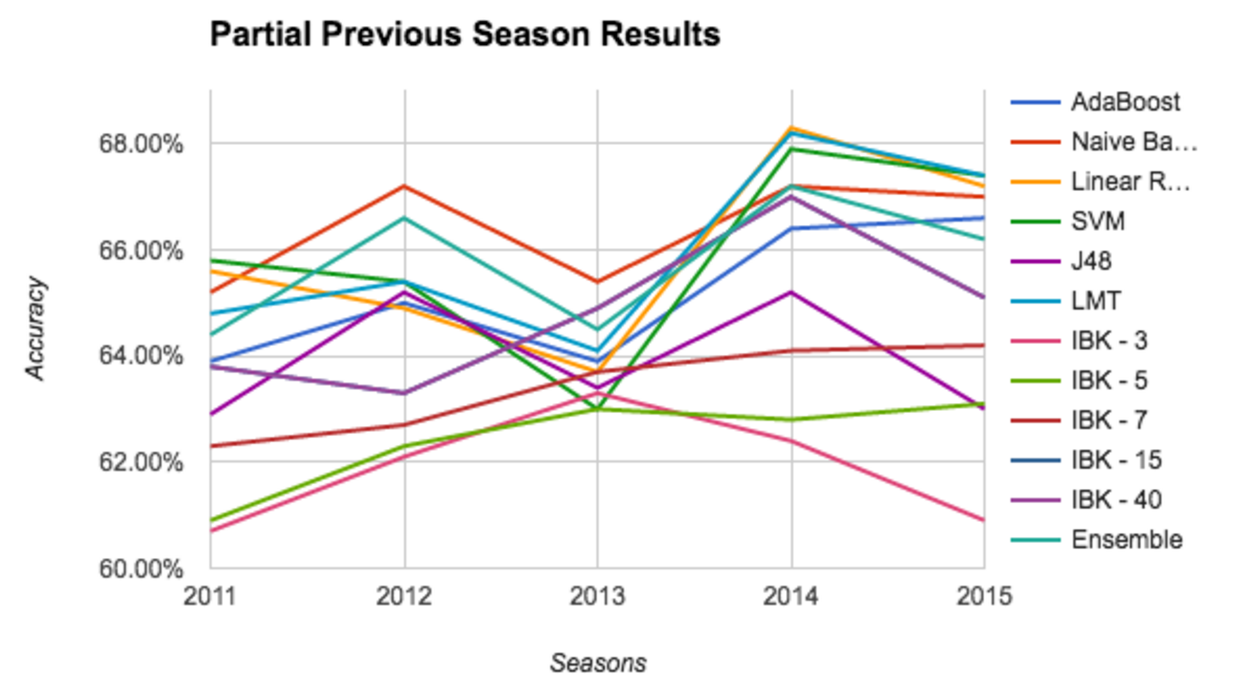
\includegraphics[scale=0.7]{images/partialPreviousGraph.png}

Next are the results for full previous season training. In 2011, the ensemble method had the highest accuracy with 65.6\%. In 2012, the best classifier was the Naive Bayes with an accuracy of 66.7\%. In 2013, K-Nearest Neighbors outperformed others with 65.9\% accuracy for both 15 and 40 neighbors respectively. In 2014, both LMT and SVM tied for the best accuracy with 68.2\%. Finally, in 2015, Linear Regression was the best algorithm with an accuracy of 68\%. One observation we made in this round of experiments was that the K-Nearest Neighbors algorithm had the exact same accuracy for both K = 15 and K = 40 for each season. This turned out to be true in the last round of experiments as well.

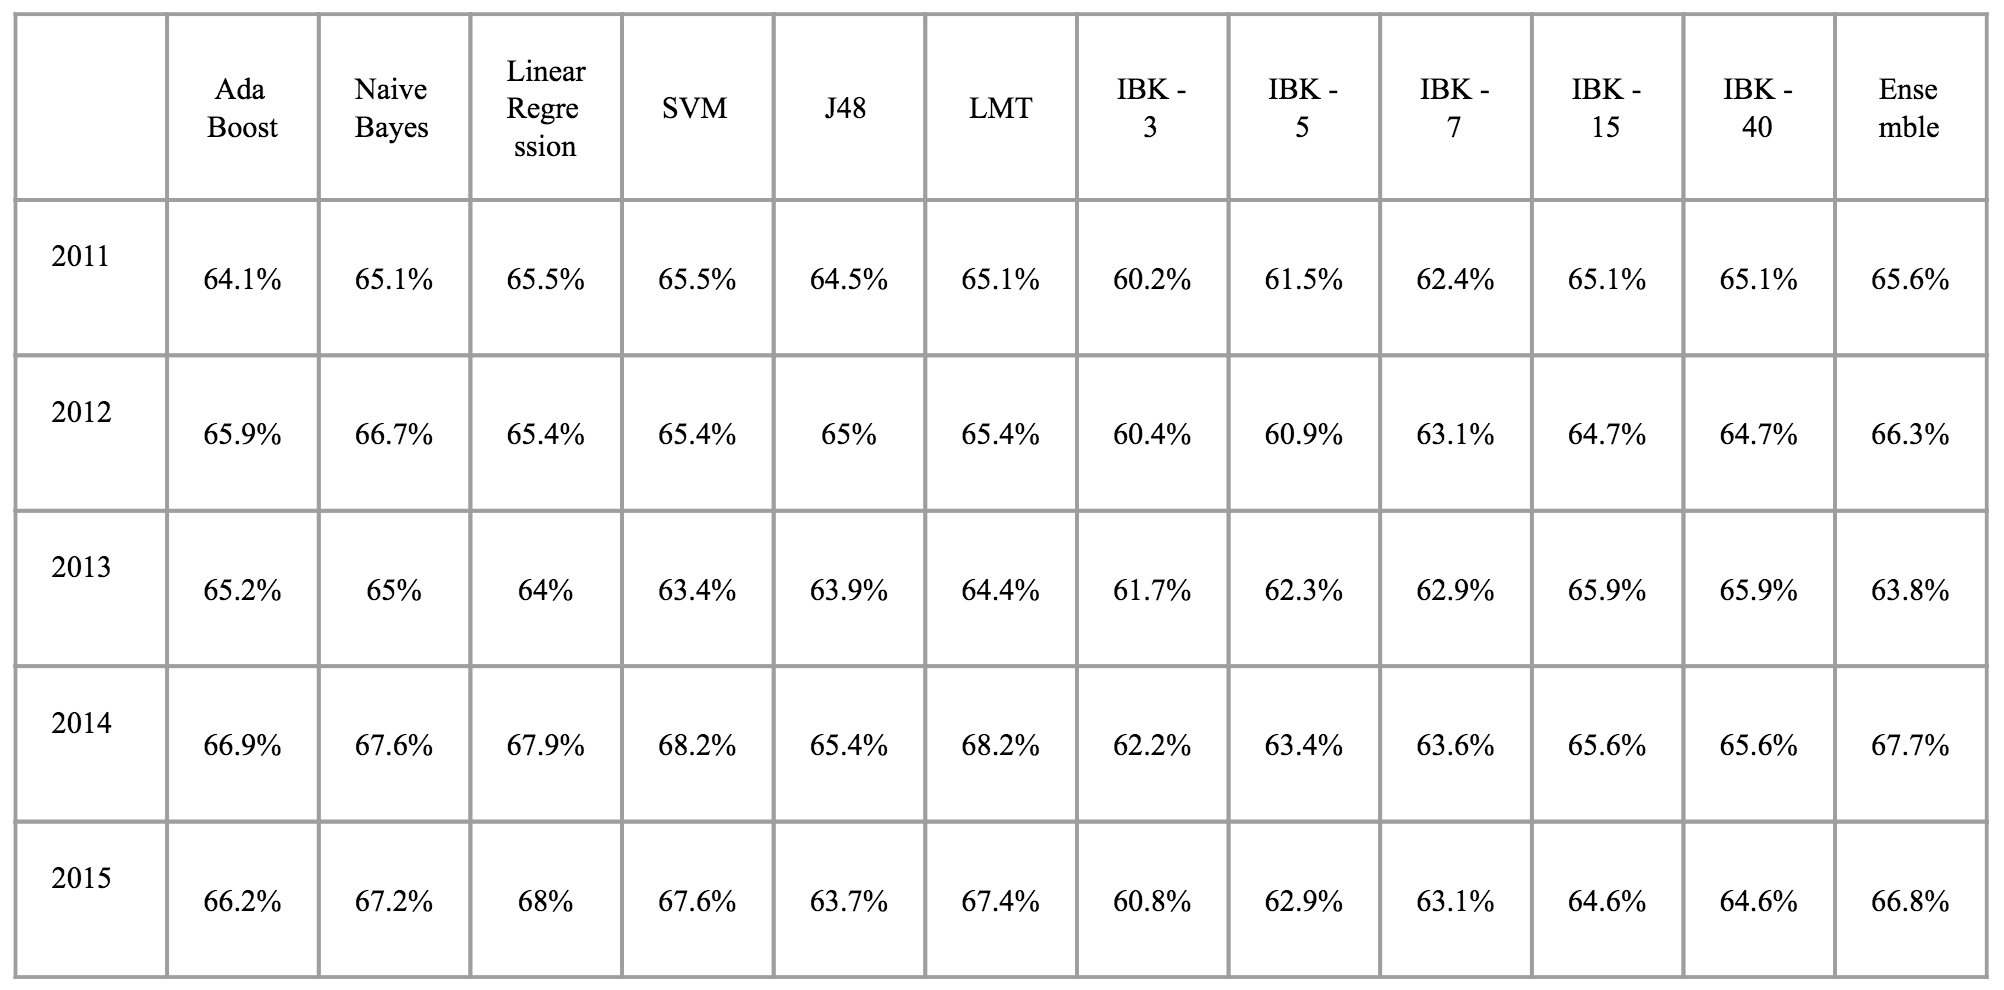
\includegraphics[scale=0.405]{images/fullPrevResults.png}

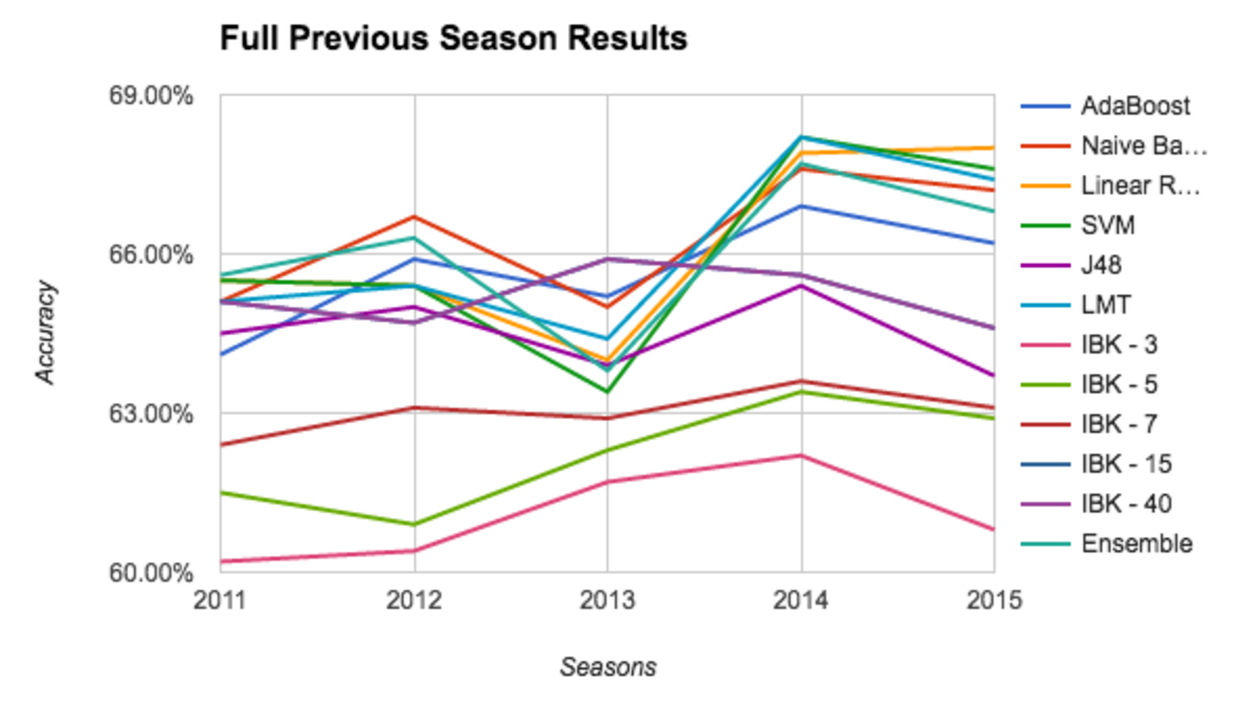
\includegraphics[scale=0.7]{images/fullPreviousGraph.png}

In the final set, we added injury data into the set of features. In 2011, the SVM had the highest accuracy with 65.7\%. In 2012, AdaBoost had the highest accuracy with 66.4\%. Finally, in 2013, Naive Bayes had the highest accuracy with 65.9\%. Here, K-Nearest Neighbors with K = 40 performed better in a single instance than the same algorithm with K = 15. The overwhelming conclusion is either that injuries do not have any discernable effect on team performance (unlikely) or that our method of measure the effect of injuries is not adequate. This topic is further discussed in the future work section.

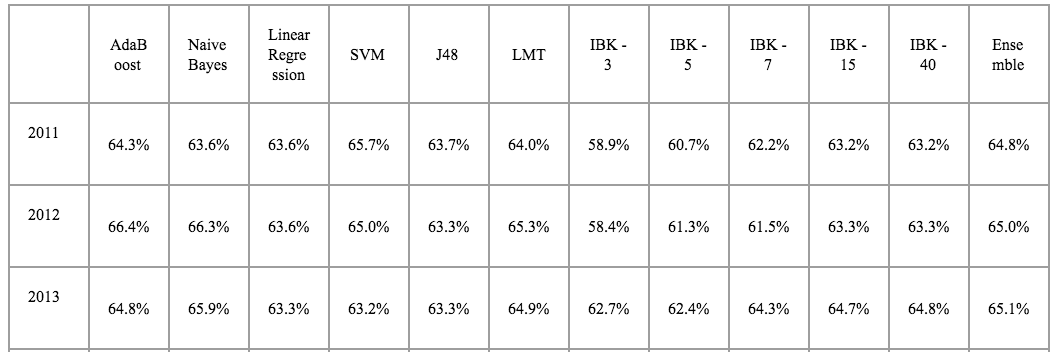
\includegraphics[scale=0.8]{images/injuryData.png}

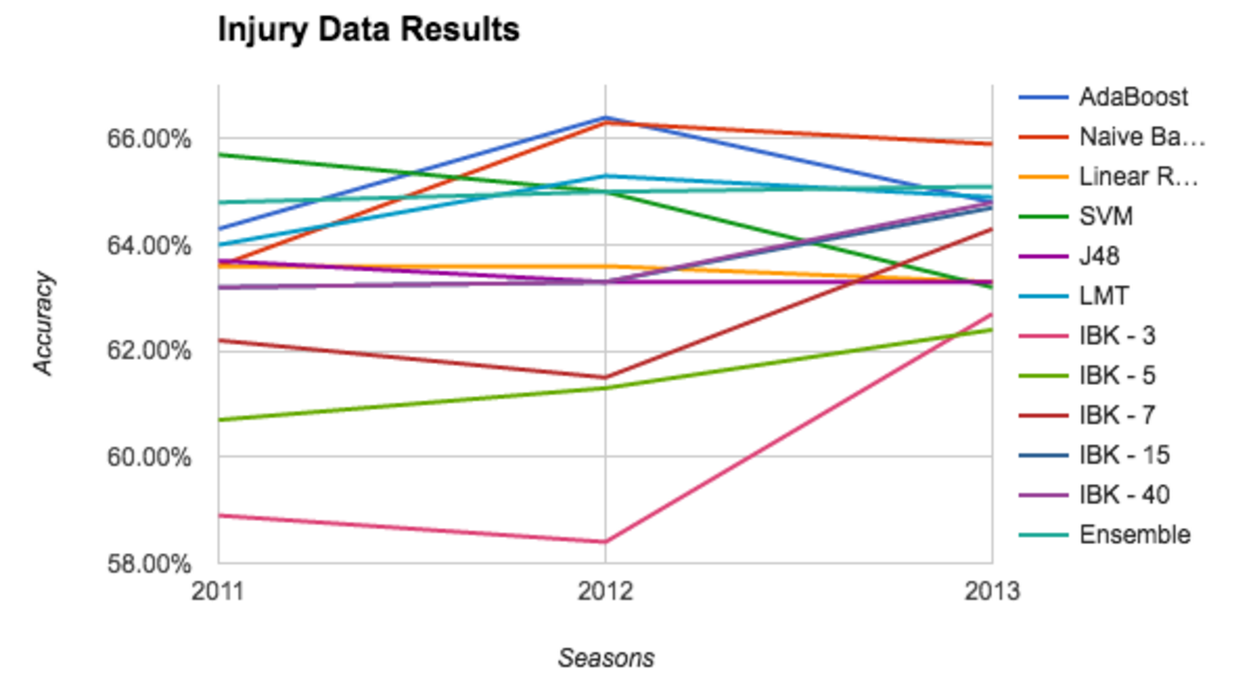
\includegraphics[scale=0.7]{images/injuryGraph.png}

Overall, our results were in line with many of the papers we discovered online during the initial stages of the project. In general, no classifier breaks into 70\% accuracy with the data that we are using to train and test. While this is better than flipping a coin, we are still interested in finding ways to improve the accuracy of the classifiers. We found that for this type of data, the Logistic Model Tree, Support Vector Machine and Naive Bayes provided the most consistent high accuracy predictions. The ensemble method also performed worse than we predicted.

\section{Future Work}

As explained in the results section, the injury count did not significantly change the performance of the classifiers. One explanation is that the number of injured players does not take into account the importance of the missing players. Calculating the importance a single player would involve analyzing their point contribution over the course of their career on their current team. Next, each player on the team would receive an importance score based on how much they contributed in the season relative to their teammates. A simple method would be dividing the contribution of each player by the sum of points scored during the season. Once an importance metric is in place, we can numerically determine how much a team can be affected by missing players as a feature for each team in a match. Unfortunately, we did not have time accomplish this for our current project. However, we have all the data necessary to finish it in the future. 

\section*{References}

\small

[1] Renato Amorim Torres. Prediction of NBA games based on Machine Learning Methods. Project report. (2013), http://homepages.cae.wisc.edu/~ece539/fall13/project/AmorimTorres\_rpt.pdf.

[2] Matthew Beckler, Hongfei Wang. NBA Oracle. Project report. (2008), http://www.mbeckler.org/coursework/2008-2009/10701\_report.pdf.

[3] Lori Hoffman, Maria Joseph. A Multivariate Statistical Analysis of the NBA. Project Report. (2003), http://www.units.miamioh.edu/sumsri/sumj/2003/NBAstats.pdf.

[4] I. H. Witten and E. Frank. 2005. Data mining: Practical machine learning tools and techniques. (2005). http://www.cs.waikato.ac.nz/ml/weka/index.html

[5] Colet, E. and Parker, J. Advanced Scout: Data mining and knowledge discovery in NBA data. Data Mining and Knowledge Discovery, Vol. 1, Num. 1, 1997, pp 121 -- 125.

[6] Orendorff, David, and Johnson, Todd. First-Order Probabilistic Models for Predicting the Winners of Professional Basketball Games. Project report. http://www.ics.uci.edu/dorendor/basket.pdf

[7] Babak, Hamadani. Predicting the outcome of NFL games using machine learning. Project Report for CS229, Stanford University. http://www.stanford.edu/class/cs229/proj2006/BabakHamadaniPredictingNFLGames.pdf

\end{document}